\documentclass[a4paper,12pt]{article}
\usepackage[polish]{babel}
\usepackage[utf8]{inputenc}
\usepackage[T1]{fontenc}
\usepackage{lmodern}
\usepackage[top=3cm,bottom=2.5cm,left=3cm,right=3cm]{geometry}
\usepackage{graphicx}
\usepackage{url}
\usepackage{amsmath}
\usepackage{amssymb}
\usepackage{float}
\usepackage{enumitem}

\begin{document}
\begin{titlepage}
  \thispagestyle{empty}
  \begin{center}
    % --- GÓRA ---
    {\LARGE\bfseries Sztuczna inteligencja\par}
    \vspace{1.5cm}

    % --- ŚRODEK: podtytuł ---
    {\large Uczenie ze wzmocnieniem:\\
    Projekt i implementacja autonomicznego agenta gry Snake wykorzystującego\\
    Q-learning oraz sieci neuronowe\par}
    \vspace{3cm}

    % --- Autor ---
    {\Large Autor:\\
    Kacper Hyliński\par}
    {\large kierunek Informatyka\par}
    \vfill

    % --- STOPKA ---
    {\large Rzeszów, 2025\par}
    \vspace{0.4cm}
    {\normalsize Wydział Elektrotechniki i Informatyki\par}
    {\normalsize Politechnika Rzeszowska im.\ Ignacego Łukasiewicza\par}
  \end{center}
\end{titlepage}
 
 \clearpage
  \pagenumbering{roman}
  \thispagestyle{empty}
  \tableofcontents
  \clearpage
  \pagenumbering{arabic}

  \section{Cel projektu}
Celem niniejszego projektu jest opracowanie, implementacja oraz porównawcza analiza dwóch metod uczenia ze wzmocnieniem w zmodyfikowanym środowisku gry Snake, w którym agent ponosi karę za kolizję ze ścianami. W pierwszym podejściu zastosowano klasyczny algorytm Q-learning, natomiast w drugim – jego rozszerzenie o głęboką sieć neuronową (Deep Q-Network, DQN).

W ramach projektu zostanie utworzone środowisko symulacyjne, w którym agent będzie zobligowany do identyfikacji kluczowych elementów otoczenia, takich jak obszary zagrożenia oraz źródła pożywienia, a następnie do podejmowania decyzji na podstawie obserwowanych stanów. Ponadto zaimplementowany zostanie wariant Double DQN, a proces uczenia zostanie przyspieszony poprzez integrację technologii CUDA, z zapewnieniem możliwości alternatywnego przeprowadzenia treningu na procesorze centralnym w przypadku braku wsparcia GPU.

Dla optymalizacji przebiegu treningu opracowany zostanie również uproszczony interfejs gry, pozbawiony renderowania graficznego na ekranie, co pozwoli na znaczące zwiększenie efektywności procesu uczenia.
\clearpage  
\section{Część teoretyczna}
\subsection{Model neuronu}
\begin{figure}[h!]
    \centering
    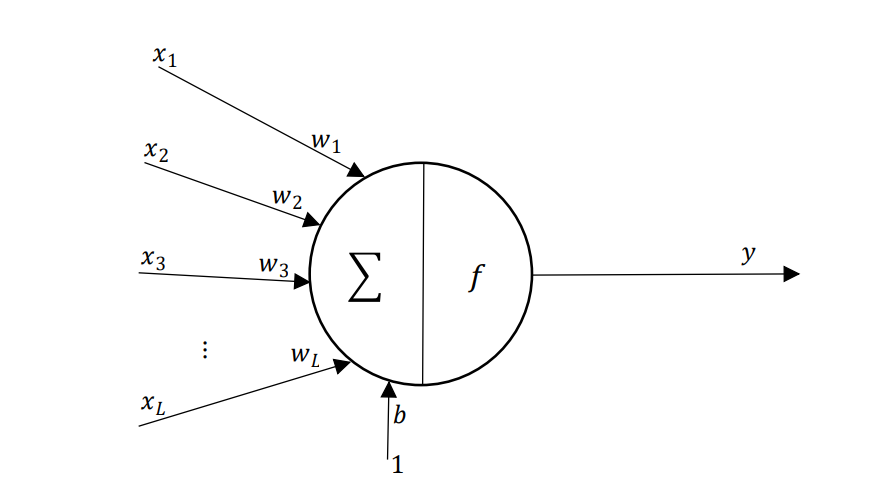
\includegraphics[width=1\linewidth]{image.png}
    \caption{Model Neuronu \cite{RZajdelNeuron}.}
\end{figure}

\noindent $\boldsymbol{x_1 - x_L}$ - sygnał wejściowy, \newline
 $\boldsymbol{w_1 - w_L}$ - współczynnik wagowy, \newline
$\boldsymbol{b}$ - bias, \newline
$\boldsymbol{\sum}$  - sumator, \newline
$\boldsymbol{f}$ - funkcja aktywująca, \newline
$\boldsymbol{y}$ - wartość wyjściowa 
\begin{equation}
y = f\Bigl(\sum_{j=1}^{L} w_j\,\cdot x_j + b\Bigr)
\end{equation}
Symbol \(x_j\) oznacza \(j\)-ty sygnał wejściowy (\(j = 1, 2, \dots, L\)), natomiast \(w_j\) odpowiada przypisanej mu wadze.

\medskip

Sumę ważoną sygnałów wejściowych wraz z wartością przesunięcia (biasu) określa się mianem \textit{łącznego pobudzenia neuronu}, które w dalszej części oznaczane będzie symbolem \(z\):
\begin{equation}
z = \sum_{j=1}^{L} w_j \cdot x_j + b.
\end{equation}


\subsection{Sieć neuronowa wielowarstwowa (MLP)}

\begin{figure}[h!]
    \centering
    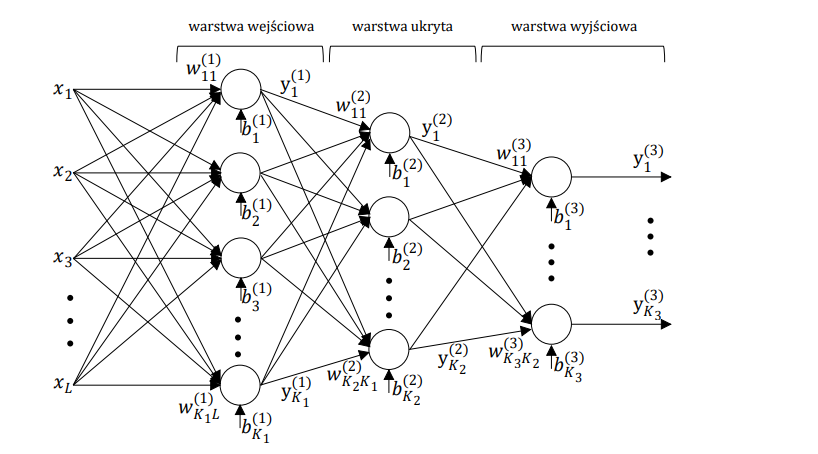
\includegraphics[width=1\linewidth]{MLP.png}
    \caption{Sieć jednokierunkowa wielowarstwowa \cite{RZajdelMLP}.}
\end{figure}

Taką sieć nazywa się trójwarstwową. Występują tu połączenia pomiędzy warstwami neuronów typu każdy z każdym.  
Sygnały wejściowe podawane są do warstwy wejściowej neuronów, których wyjścia stanowią sygnały źródłowe dla kolejnej warstwy.  
Można wykazać, że sieć trójwarstwowa nieliniowa jest w stanie odwzorować praktycznie dowolne odwzorowanie nieliniowe.

Każda warstwa neuronów posiada swoją macierz wag \(\mathbf{w}\), wektor przesunięć \(\mathbf{b}\), funkcję aktywacji \(f\) i wektor sygnałów wyjściowych \(\mathbf{y}\).  
Aby je rozróżniać w dalszych rozważaniach, do każdej z wielkości dodano numer warstwy, której dotyczą.  
Na przykład dla warstwy drugiej (ukrytej) macierz wag oznaczana będzie symbolem \(\mathbf{w}^{(2)}\).  
Działanie każdej z warstw można rozpatrywać oddzielnie.  
I tak np. warstwa druga posiada: \(L = K_1\) sygnałów wejściowych, \(K = K_2\) neuronów i macierz wag \(\mathbf{w} = \mathbf{w}^{(2)}\) o rozmiarach \(K_2 \times K_1\).  
Wejściem warstwy drugiej jest wyjście warstwy pierwszej \(\mathbf{x} = \mathbf{y}^{(1)}\), a wyjściem \(\mathbf{y} = \mathbf{y}^{(2)}\).  
Działanie poszczególnych warstw dane jest przez

\begin{equation}
y^{(1)} = f^{(1)}\left(w^{(1)}x + b^{(1)}\right), 
\end{equation}
\begin{equation}
y^{(2)} = f^{(2)}\left(w^{(2)}y^{(1)} + b^{(2)}\right), 
\end{equation}
\begin{equation}
y^{(3)} = f^{(3)}\left(w^{(3)}y^{(2)} + b^{(3)}\right).
\end{equation} 

Działanie całej sieci można więc opisać jako
\begin{equation}
\mathbf{y}^{(3)} = f^{(3)}\left( \mathbf{w}^{(3)} f^{(2)}\left( \mathbf{w}^{(2)} f^{(1)}\left( \mathbf{w}^{(1)} \mathbf{x} + \mathbf{b}^{(1)} \right) + \mathbf{b}^{(2)} \right) + \mathbf{b}^{(3)} \right).
\end{equation}

\cite{RZajdelMLP}



W projekcie Snake AI do aproksymacji funkcji wartości $Q(s,a)$ wykorzystujemy wielowarstwową sieć neuronową (MLP) o strukturze:

\begin{itemize}
\item Warstwa wejściowa: wymiar wektora stanu $d=11$ cech,
\item trzy warstwy ukryte:
\begin{itemize}
\item pierwsza z $H_1=256$ neuronów,
\item druga z $H_2=256$ neuronów,
\item trzecia z $H_3 = 128$ neuronów,
\end{itemize}
\item Warstwa wyjściowa: liczba wyjść równa liczbie akcji $|A|=3$.
\end{itemize}

\subsection{MLP w projekcie Snake AI}
W projekcie Snake AI do aproksymacji funkcji wartości Q(s,a) wykorzystujemy wielowarstwową sieć neuronową (MLP) składającą się z warstwy wejściowej, dwóch warstw ukrytych i warstwy wyjściowej. 

\begin{equation}
\mathbf{y}^{1} = f^{1}(\mathbf{z}^{1}) = f^{1}(\mathbf{w}^{1} \mathbf{x} + \mathbf{b}^{1}) 
\end{equation}
\begin{equation}
\mathbf{y}^{2} = f^{2}(\mathbf{z}^{2}) = f^{2}(\mathbf{w}^{2} \mathbf{y}^{1} + \mathbf{b}^{2}) 
\end{equation}
\begin{equation}
\mathbf{y}^{3} = f^{3}(\mathbf{z}^{3}) = f^{3}(\mathbf{w}^{3} \mathbf{y}^{2} + \mathbf{b}^{3}) 
\end{equation}
\begin{equation}
\mathbf{y}^{4} = f^{4}(\mathbf{z}^{4}) = f^{4}(\mathbf{w}^{4} \mathbf{y}^{3} + \mathbf{b}^{4})
\end{equation}

Gdzie \(f^{1}, f^{2}, f^{3}\) to funkcje Leaky ReLU, a \(f^{4}\) to funkcja liniowa.

\textit{wzór opisujący działanie całej sieci jako złożenie funkcji:}

\begin{equation}
\mathbf{y}^{4} = f^{4}\left( \mathbf{w}^{4} f^{3} \left( \mathbf{w}^{3} f^{2} \left( \mathbf{w}^{2} f^{1}(\mathbf{w}^{1} \mathbf{x} + \mathbf{b}^{1}) + \mathbf{b}^{2} \right) + \mathbf{b}^{3} \right) + \mathbf{b}^{4} \right)
\end{equation}

\subsection{Funkcje aktywacji}

W ramach niniejszego projektu, którego celem jest implementacja agenta Deep Q-Network (DQN) w środowisku gry Snake, zastosowano różne funkcje aktywacji. Ich dobór został przeprowadzony w sposób celowy i dostosowany do charakterystyki poszczególnych warstw sieci neuronowej.

\textbf{Leaky ReLU} – funkcja aktywacji, która wprowadza niewielki współczynnik nachylenia dla wartości ujemnych, co pozwala na uniknięcie problemu zanikania gradientu i „martwych neuronów”. Funkcja ta jest zdefiniowana jako:
\begin{equation}
f(x) = \begin{cases}
x & \text{jeśli } x > 0 \\
\alpha x & \text{jeśli } x \leq 0
\end{cases}
\end{equation}

lub w bardziej zwartej postaci:
\[
f(x) = \max(\alpha x, x),
\]
gdzie \(\alpha\) to mała wartość (w naszym projekcie \(0{,}01\)), która kontroluje nachylenie dla wartości ujemnych. W sieci DQN używamy Leaky ReLU we wszystkich warstwach ukrytych.

\medskip

\textbf{Funkcja liniowa} – funkcja aktywacji używana w warstwie wyjściowej sieci DQN, która nie wprowadza żadnej nieliniowości, co pozwala na nieograniczony zakres wartości wyjściowych. Jest zdefiniowana jako:
\begin{equation}
f(x) = x
\end{equation}

Funkcja ta jest szczególnie przydatna w warstwie wyjściowej sieci aproksymującej funkcję \(Q\), gdzie wyjścia mogą przyjmować dowolne wartości rzeczywiste.

\begin{figure}[H]
    \centering
    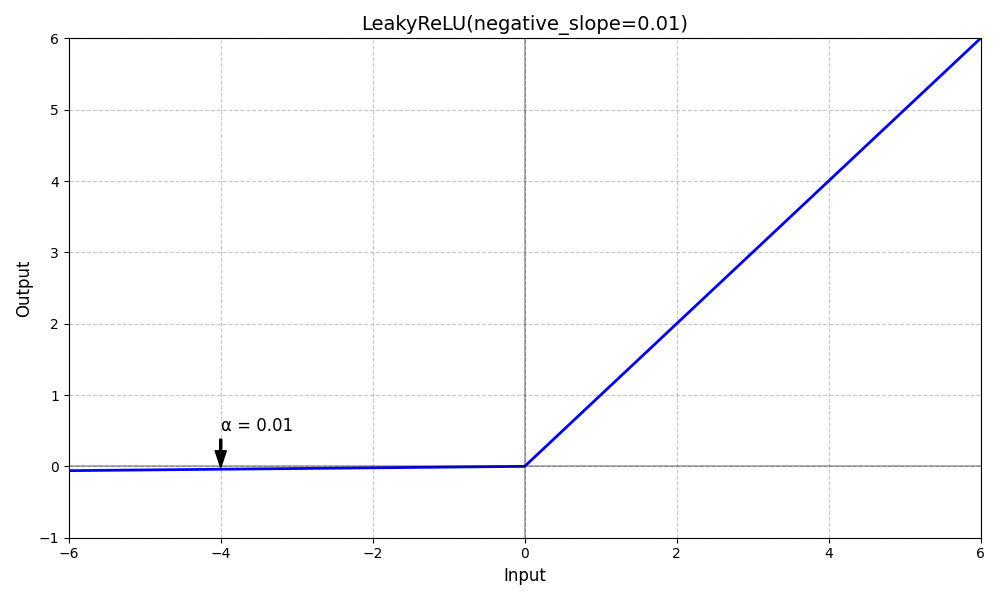
\includegraphics[width=1\linewidth]{LeakyRelu.png}
    \caption{Wykres LeakyRelu}
\end{figure}

Funkcja liniowa w warstwie wyjściowej sieci DQN została wybrana ze względu na następujące właściwości i zalety:

\begin{enumerate}[label=\textbf{\arabic*.}, leftmargin=1.5cm]
    \item \textbf{Nieograniczony zakres wartości wyjściowych} – w kontekście aproksymacji funkcji wartości \(Q\), wyjścia sieci mogą przyjmować dowolne wartości rzeczywiste. Funkcja liniowa nie wprowadza żadnych ograniczeń zakresu wartości wyjściowych, co jest kluczowe dla poprawnego przewidywania wartości funkcji \(Q\) \cite{mnih2015human}.

    \item \textbf{Zgodność z teorią DQN} – w oryginalnej publikacji opisującej algorytm Deep Q-Network autorstwa Mnih et al. (2015), również zastosowano liniową funkcję aktywacji w warstwie wyjściowej, co potwierdza zasadność wyboru tego rozwiązania \cite{mnih2015human}.

    \item \textbf{Rozwiązanie problemu "umierających neuronów":} Standardowa funkcja ReLU zwraca 0 dla wszystkich wartości ujemnych, co może prowadzić do "umierania neuronów", kiedy neuron zawsze daje wartość 0 na wyjściu. LeakyReLU rozwiązuje ten problem, pozwalając na przepływ małego gradientu dla wartości ujemnych.
\end{enumerate}

\clearpage 

\subsection{Wprowadzenie do uczenia ze wzmocnieniem i MDP}
Uczenie ze wzmocnieniem (ang.\ \emph{Reinforcement Learning}, RL) to rodzaj uczenia maszynowego, w którym agent uczy się podejmować sekwencje decyzji poprzez interakcję ze środowiskiem. Po każdej akcji podjętej w stanie środowiska agent otrzymuje \emph{nagrodę} – skalarny feedback – i przechodzi do nowego stanu. Celem agenta jest opracowanie \emph{strategii (polityki)} wyboru akcji maksymalizującej skumulowaną nagrodę w długim horyzoncie czasowym.

Formalnie środowisko modeluje się jako \emph{proces decyzyjny Markowa} (MDP), zdefiniowany jako krotka
\[
\mathcal{M} = (\mathcal{S}, \mathcal{A}, P, R),
\]
gdzie:
\begin{itemize}
  \item $\mathcal{S}$ – zbiór stanów,
  \item $\mathcal{A}$ – zbiór akcji,
  \item $P: \mathcal{S}\times\mathcal{A}\times\mathcal{S}\to[0,1]$, \quad
        $P(s' \mid s,a)=\Pr(s_{t+1}=s'\mid s_t=s,\,a_t=a)$ – funkcja przejścia definiująca rozkład prawdopodobieństwa kolejnego stanu,
  \item $R: \mathcal{S}\times\mathcal{A}\to\mathbb{R}$, \quad
        $R(s,a)=\mathbb{E}[r_{t+1}\mid s_t=s,\,a_t=a]$ – funkcja nagród.
\end{itemize}

Jeśli w chwili $t$ agent znajduje się w stanie $s_t$ i wybierze akcję $a_t$, to z prawdopodobieństwem 
$P(s_{t+1}=s'\mid s_t,a_t)$ przejdzie do stanu $s_{t+1}=s'$ i otrzyma nagrodę 
$r_{t+1}=R(s_t,a_t)$. Proces ten powtarza się iteracyjnie, tworząc ścieżkę stanów, akcji i nagród. 
Sumaryczna zdyskontowana nagroda od chwili $t$ jest zwykle definiowana jako
\[
R_t \;=\; \sum_{k=0}^{\infty} \gamma^k\,r_{t+k+1},
\]
gdzie $\gamma\in[0,1]$ to współczynnik dyskontowania.

gdzie \(0 \le \gamma < 1\) to współczynnik dyskontowania określający ważność przyszłych nagród.\footnote{Niższa wartość \(\gamma\) sprawia, że agent przywiązuje większą wagę do nagród natychmiastowych niż odległych w czasie.} Formalnym celem uczenia ze wzmocnieniem jest znalezienie strategii \(\pi^*\), która maksymalizuje wartość oczekiwaną powyższej sumy nagród.

\subsection*{Funkcja wartości}
Kluczową koncepcją w uczeniu ze wzmocznieniem jest \emph{funkcja wartości}. Dla danej strategii \(\pi\) definiujemy wartość stanu
\[
V^{\pi}(s)
= \mathbb{E}\Bigl[\sum_{k=0}^\infty \gamma^k\,r_{t+k+1}\;\Bigm|\;s_t=s\Bigr].
\]
Analogicznie \emph{funkcję wartości akcji} określa się jako
\[
Q^{\pi}(s,a)
= \mathbb{E}\bigl[r_{t+1} + \gamma\,Q^{\pi}\bigl(s_{t+1},\pi(s_{t+1})\bigr)\;\bigm|\;s_t=s,\,a_t=a\bigr].
\]
Równanie to (zwane \emph{równaniem Bellmana} dla \(Q^\pi\)) wyraża zależność wartości akcji od natychmiastowej nagrody oraz wartości przyszłego stanu. 

Dla strategii optymalnej \(\pi^*\), maksymalizującej zdyskontowaną nagrodę, zachodzi \emph{równanie optymalności Bellmana}:
\[
Q^*(s,a)
= r(s,a) + \gamma \sum_{s'} P(s'\mid s,a)\,\max_{a'} Q^*(s',a').
\]

gdzie \(Q^*(s,a)\) oznacza optymalną funkcję wartości akcji. Innymi słowy, zakładając znajomość pełnego modelu środowiska \((P,R)\), \(Q^*\) spełnia układ równań, z którego (przynajmniej teoretycznie) da się wyznaczyć optymalne wartości i strategię:
\[
\pi^*(s) \;=\; \arg\max_{a} Q^*(s,a).
\]
W praktyce jednak model środowiska często nie jest znany lub zbyt złożony, a przestrzeń stanów ogromna, dlatego stosujemy metody iteracyjne i przybliżone, aby oszacować \(Q^*\).

\subsection{Klasyczny algorytm Q-learning}

Q-learning jest jedną z najpopularniejszych metod uczenia ze wzmocnieniem typu \emph{off-policy} wykorzystujących różnice czasowe. Algorytm ten potrafi uczyć się bezpośrednio na podstawie doświadczeń z interakcji, nie znając apriori funkcji przejścia ani nagród. Zbieżność Q-learningu do optymalnych wartości~$Q^*$ została udowodniona w przypadku dyskretnych przestrzeni stanów i akcji przy odpowiednich założeniach (m.in.\ że każda para stan–akcja jest odwiedzana nieskończenie często, a współczynnik uczenia maleje w czasie).

Algorytm utrzymuje estymację funkcji wartości akcji~$Q(s,a)$ w postaci tabelarycznej (tablicy wartości dla każdej pary stan–akcja). Początkowo przypisuje się jej pewne wartości (np.\ losowe lub zerowe). Następnie agent rozgrywa serię epizodów interakcji ze środowiskiem. W każdym kroku epizodu ze stanu~$s_t$ wybierana jest akcja~$a_t$ zgodnie z aktualną strategią eksploracyjno–eksploatacyjną. Najczęściej stosuje się strategię~$\varepsilon$-greedy, w której z prawdopodobieństwem~$1-\varepsilon$ wybierana jest akcja optymalna według bieżących wartości~$Q$, a z prawdopodobieństwem~$\varepsilon$ agent eksploruje, wybierając akcję losową. Pozwala to uniknąć „uwięzienia” w polityce zachłannej opartej na niedokładnych wartościach i zapewnia odwiedzanie różnych stanów. Parametr~$\varepsilon$ (np.\ początkowo~1) często zmniejsza się w miarę uczenia, aby eksploracja malała z czasem na rzecz eksploatacji zdobytej wiedzy.

Po podjęciu akcji~$a_t$ w stanie~$s_t$ i otrzymaniu nagrody~$r_t$ oraz obserwacji nowego stanu~$s_{t+1}$ następuje aktualizacja oceny $Q(s_t,a_t)$. Klasyczny Q-learning wykorzystuje w tym celu błąd przewidywania, tzw.\ błąd TD (temporal difference), definiowany jako:
\[
\delta = r + \gamma \max_{a'} Q(s',a') \;-\; Q(s,a).
\]

Błąd TD wyraża różnicę między aktualną estymacją wartości \(Q(s,a)\) a wartością docelową
\[
y = r + \gamma \max_{a'} Q(s',a'),
\]
opartą na bieżących ocenach stanu następnego. Następnie wartość \(Q(s,a)\) jest przesuwana w kierunku wartości docelowej o krok proporcjonalny do współczynnika uczenia \(\alpha\) (zwykle \(\alpha \in [0,1]\)):
\[
Q(s,a) \;\leftarrow\; Q(s,a) + \alpha\bigl[r + \gamma \max_{a'} Q(s',a') \;-\; Q(s,a)\bigr].
\]
Powyższa reguła aktualizacji jest implementacją iteracji Bellmana na podstawie pojedynczych doświadczeń. Intuicyjnie, jeśli zaobserwowana natychmiastowa nagroda \(r\) wraz z najlepszą przewidywaną wartością przyszłą \(\max_{a'} Q(s',a')\) przewyższa dotychczasową ocenę \(Q(s,a)\), to \(Q(s,a)\) zostanie zwiększone (i odwrotnie – przeszacowane wartości są zmniejszane). Współczynnik \(\alpha\) reguluje szybkość uczenia: małe \(\alpha\) sprawia, że wartości zmieniają się wolniej (co uśrednia wiele doświadczeń), natomiast \(\alpha = 1\) oznacza całkowite zastąpienie starej wartości nowym jednorazowym oszacowaniem. Dzięki niezależności aktualizacji od konkretnej strategii wyboru akcji (algorytm off-policy), Q-learning w teorii konwerguje do \(Q^*\) nawet jeśli podczas uczenia agent nie zawsze podąża strategią zachłanną.

Algorytm Q-learning stopniowo poprawia przybliżenia wartości akcji. Z czasem, gdy \(Q(s,a)\) zbliża się do wartości optymalnych, strategia zachłanna względem tych wartości staje się strategią optymalną \(\pi^*\). W praktyce tablicowy Q-learning jest stosowany tylko dla stosunkowo niewielkich i dyskretnych przestrzeni stanów, ponieważ przechowywanie i aktualizacja tablicy \(Q(s,a)\) w większych problemach (np.\ gdy stanem jest obraz Atari) jest niewykonalne. Rozwiązaniem problemu skalowalności jest zastąpienie tablicy \(Q\) funkcją przybliżającą – tu z pomocą przychodzi sieć neuronowa\(^*\).

\subsection{Deep Q-Network (DQN)}

Deep Q-Network (DQN) to algorytm, który łączy klasyczny Q-learning z możliwościami głębokich sieci neuronowych do aproksymacji funkcji wartości \(Q\). Fundamentalna koncepcja polega na zastąpieniu tablicy \(Q(s,a)\) przez sieć neuronową \(Q(s,a;\theta)\) parametryzowaną wektorem \(\theta\). Sieć przyjmuje na wejściu reprezentację stanu \(s\) i generuje na wyjściu estymowane wartości \(Q(s,a)\) dla zbioru dostępnych akcji. Dzięki temu podejściu algorytm uzyskuje zdolność skalowania do rozległych (w tym ciągłych) przestrzeni stanów, realizując generalizację – tj. aproksymując podobne wartości dla stanów wykazujących wspólne cechy, co pozostaje poza zasięgiem tablicowego Q-learningu.
W implementacji DQN przyjęto strukturę czterowarstwowej sieci neuronowej typu MLP (Multi-Layer Perceptron).

\subsubsection*{Metodologia treningu}

Proces uczenia sieci \(Q(s,a;\theta)\) opiera się na minimalizacji różnicy między predykcjami a wartościami docelowymi obliczanymi na podstawie ewaluacji stanu środowiska (analogicznie do procedury w tablicowym Q-learningu). W każdej iteracji procesu uczenia analizowana jest próbka doświadczenia \((s,a,r,s',done)\), na podstawie której wyznaczana jest wartość docelowa:
\[
y = r + \gamma \max_{a'} Q(s',a';\theta^-) \cdot (1 - done),
\]
gdzie \(\theta^-\) oznacza parametry sieci docelowej, a \(done\) stanowi indykator stanu terminalnego (tj. zakończenia epizodu). 

W opisywanej implementacji zastosowano modyfikację algorytmu DQN określaną jako Double DQN, która adresuje problem systematycznego przeszacowania wartości Q. W standardowym DQN ta sama sieć wykorzystywana jest zarówno do selekcji, jak i ewaluacji akcji, co może skutkować zawyżaniem wartości Q. W paradygmacie Double DQN sieć główna dokonuje selekcji akcji, natomiast sieć docelowa przeprowadza jej ewaluację:
\[
y = r + \gamma \cdot Q(s', \arg\max_{a'} Q(s',a';\theta); \theta^-) \cdot (1 - done)
\]

Następnie definiowana jest funkcja straty. W implementacji wykorzystano funkcję Hubera (operacyjnie zaimplementowaną jako SmoothL1Loss w bibliotece PyTorch), która charakteryzuje się zwiększoną odpornością na wartości odstające w porównaniu do błędu średniokwadratowego:
\[
\mathcal{L}_\delta(\theta) =
\begin{cases}
\tfrac12\bigl(y - Q(s,a;\theta)\bigr)^2, & \text{jeśli } |y - Q(s,a;\theta)| \le \delta,\\
\delta\bigl(|y - Q(s,a;\theta)| - \tfrac12\delta\bigr), & \text{jeśli } |y - Q(s,a;\theta)| > \delta.
\end{cases}
\]
gdzie \(\delta\) stanowi parametr delimitujący przejście między kwadratową a liniową charakterystyką funkcji straty (przyjęto \(\delta=1\)). Funkcja Hubera zapewnia, że dla znacznych odchyleń model nie generuje nieograniczonych wartości gradientu (jak ma to miejsce w funkcji MSE), co zabezpiecza przed niestabilnością uczenia wywołaną zjawiskiem eksplozji gradientów. 

W implementacji wykorzystano optymalizator Adam (w przypadku obliczeń na CPU) lub AdamW (w przypadku obliczeń na GPU) ze współczynnikiem uczenia \(\alpha=0.0003\). AdamW wprowadza regularyzację typu Weight Decay, co przyczynia się do zwiększenia stabilności procesu uczenia na architekturach GPU. Dodatkowo zastosowano technikę przycinania gradientów (gradient clipping) do normy jednostkowej, co stanowi kolejny mechanizm stabilizujący proces treningu.

\subsubsection*{Mechanizm Experience Replay}

Kluczowym komponentem architektury DQN jest mechanizm Experience Replay, który gromadzi doświadczenia agenta w buforze pamięci i realizuje losowe próbkowanie podczas procesu uczenia. W prezentowanej implementacji zastosowano bufor doświadczeń o pojemności \(5 \cdot 10^4\) przejść. W każdej iteracji uczenia losowany jest mini-batch o liczności 256 (w przypadku obliczeń na GPU) lub 64 (w przypadku obliczeń na CPU) próbek, co redukuje korelację temporalną między danymi treningowymi i stabilizuje proces uczenia. 

Dodatkowo zaimplementowano optymalizację polegającą na asynchronicznym, wyprzedzającym pobieraniu batcha w odrębnym wątku obliczeniowym, co zwiększa efektywność czasową treningu. Bufor pamięci został zrealizowany jako struktura deque z ograniczoną długością maksymalną, co zapewnia automatyczną eliminację najstarszych doświadczeń po osiągnięciu założonej pojemności.

\subsubsection*{Sieć docelowa}

W celu dalszego zwiększenia stabilności procesu uczenia, architektura DQN wykorzystuje dedykowaną sieć docelową (ang. Target Network) z parametrami \(\theta^-\), która podlega periodycznej aktualizacji poprzez transfer parametrów z sieci głównej w określonych interwałach czasowych (w implementacji co \(10^3\) kroków). Takie podejście zapewnia, że wartości docelowe wykorzystywane w procesie uczenia charakteryzują się odpowiednią stałością temporalną, co istotnie stabilizuje proces uczenia.

\subsubsection*{Techniki optymalizacji obliczeniowej}

W prezentowanej implementacji algorytmu DQN wprowadzono szereg technik optymalizacji obliczeniowej celem akceleracji procesu treningu:
\begin{itemize}
\item Hybrydowy paradygmat obliczeń CPU/GPU, gdzie symulacja środowiska realizowana jest na CPU (z możliwością równoległej symulacji wielu instancji środowiska), natomiast operacje uczenia wykonywane są na GPU
\item Adaptacyjny dobór precyzji reprezentacji liczb zmiennoprzecinkowych (float16/float32) w zależności od specyfikacji dostępnej architektury GPU
\item Dynamiczna parametryzacja rozmiaru batcha w dostosowaniu do dostępnych zasobów obliczeniowych
\item Paralelizacja procesu akwizycji doświadczeń z wielu współbieżnych instancji środowiska
\end{itemize}

Zastosowane techniki optymalizacji umożliwiają znaczącą akcelerację procesu uczenia, w szczególności na systemach wyposażonych w architekturę GPU.
  \section{Analiza Danych}

  \section{Skrypt programu}

  \section{Eksperymenty}

  \section{Podsumowanie i wnioski}

\clearpage
  
\renewcommand{\refname}{Literatura}
\begin{thebibliography}{9}

\bibitem{RZajdelNeuron}
Zajdel R., \textit{Sztuczna inteligencja / Metody sztucznej inteligencji w sterowaniu, Laboratorium, Ćwiczenie 4: Model Neuronu},\\
\url{https://materialy.prz-rzeszow.pl/pracownik/pliki/34/%C4%86WICZENIE%2061.pdf}.

\bibitem{RZajdelMLP}
Zajdel R., \textit{Sztuczna inteligencja / Metody sztucznej inteligencji w sterowaniu, Laboratorium, Ćwiczenie 7: Sieć neuronowa jednokierunkowa wielowarstwowa},\\
\url{https://materialy.prz-rzeszow.pl/pracownik/pliki/34/ĆWICZENIE%209.pdf}.

\bibitem{mnih2015human}
Mnih V., Kavukcuoglu K., Silver D., Graves A., Antonoglou I., Wierstra D., Riedmiller M.,\\
\textit{Human-level control through deep reinforcement learning},\\
Nature.
\url{https://www.nature.com/articles/nature14236}.

\bibitem{harvard}
R. Sutton, A. Barto, Reinforcement Learning: An Introduction, 2nd ed., 2018. \url{https://web.stanford.edu/class/psych209/Readings/SuttonBartoIPRLBook2ndEd.pdf}

\bibitem{PolitechnikaGdańska}
Wydział Elektroniki, Telekomunikacji i Informatyki, Politechnika Gdańska, \emph{Uczenie ze wzmocnieniem – materiały wykładowe do kursu „Metody sztucznej inteligencji w sterowaniu”}, 2017, \url{https://eti.pg.edu.pl/documents/176468/53881396/UW_MSU_2017.pdf}.

\bibitem{LeakyReLU}
Leaky ReLU, \textit{Dokumentacja}, \url{https://docs.pytorch.org/docs/stable/generated/torch.nn.LeakyReLU.html} \\

\bibitem{Pytorch}
Pytorch, \textit{Dokumentacja}, \url{https://pytorch.org/docs/stable/index.html} \\



\end{thebibliography}



\end{document}
